\documentclass[11pt]{article}
\usepackage{acl2016}
\usepackage{amsmath}
\usepackage{times}
\usepackage{latexsym}
\usepackage{color}
\usepackage{booktabs}
\usepackage{subfig}
\usepackage{tikz}
\usetikzlibrary{bayesnet}

\newcommand{\secref}[1]{Section~\ref{sec:#1}}
\newcommand{\figref}[1]{Figure~\ref{fig:#1}}
\newcommand{\algref}[1]{Algorithm~\ref{alg:#1}}
\newcommand{\tabref}[1]{Table~\ref{tab:#1}}
\newcommand{\mattnote}[1]{\textcolor{red}{NOTE: #1}}
\newcommand{\blank}{\underline{\hspace{.5cm}}}
\newcommand{\lexicalpredicate}[1]{\ensuremath{\textit{#1}}}
\newcommand{\formalpredicate}[1]{\ensuremath{\textsc{#1}}}
\newcommand{\entity}[1]{\ensuremath{\textsc{#1}}}

\newcommand{\true}[0]{\formalpredicate{true}}
\newcommand{\false}[0]{\formalpredicate{false}}

%\aclfinalcopy % Uncomment this line for the final submission
%\def\aclpaperid{***} %  Enter the acl Paper ID here

\title{Open-Vocabulary Semantic Parsing\\with both Distributional
Statistics and Formal Knowledge}

\author{}%Matt Gardner and Jayant Krishnamurthy\\
%Allen Institute for Artificial Intelligence\\
%Seattle, Washington, USA\\
%{\tt \{mattg,jayantk\}@allenai.org}}

\date{}

\begin{document}

\maketitle

\begin{abstract}

  We consider the problem of mapping language onto meaning
  representations that are executable, returning truth values for
  complete statements and distributions over entities for queries.
  The typical approach to solve this problem is semantic parsing;
  however, this approach fails when the language cannot be represented
  by a single query over the Freebase schema.  Instead, our approach
  represents language as a \emph{weighted combination} of queries over
  the formal schema, along with a distributional component similar to
  a word embedding.  This technique combines the advantages of
  traditional semantic parsing (compositionality and the ability to
  leverage a structured knowledge base) with the broad coverage
  obtained by distributional methods.  We present relative gains of
  over 120\% in mean average precision versus prior work on an
  open-vocabulary fill-in-the-blank question answering task.

\end{abstract}

\section{Introduction}

How should a computer program represent the meaning of a word or a
phrase? Recent work has suggested two vastly different
approaches---distributional vector space models and semantic
parsing---each with its own advantages and disadvantages. On one hand,
distributional models produce a vector representation of the meaning
of each word from a large unlabeled text corpus. These models have
broad coverage, but only a shallow semantics centered around word
similarity. On the other hand, semantic parsing translates natural
language into logical queries against a formal knowledge base, such as
Freebase. This approach produces a rich compositional semantics and
can leverage structured information from the knowledge base. However,
semantic parsers have limited coverage as they can only represent the
meanings of words that can be mapped to knowledge base predicates. A
critical question is \emph{how do we obtain the benefits of both of
these approaches?}

\begin{figure*}[ht]
  \small
  \begin{minipage}{0.18\linewidth}
    \textbf{Input Text}\\Italian architect \blank{}
  \end{minipage}
%
  ~~ $\longrightarrow$ ~~~~~~
%
  \begin{minipage}{0.7\linewidth}
    \textbf{Logical Form}\\
    $\lambda x.\lexicalpredicate{architect}(x)~\land~\lexicalpredicate{architect\_N/N}(\entity{Italy}, x)$
  \end{minipage}

  \vspace{.2in}
  \begin{minipage}{0.5\linewidth}
    \textbf{Category models}\\
    \begin{tabular}{@{}lll}
      \lexicalpredicate{architect}: & $\theta$: &[.2, -.6, \ldots] \\
      & $\omega$: & \textsc{type:architect} $\rightarrow$ .52 \\
      &           & \textsc{type:designer} $\rightarrow$ .32 \\
      &           & \textsc{nationality:Italy} $\rightarrow$ .20 \\
      &           & $\cdots$
    \end{tabular}
  \end{minipage}
  \begin{minipage}{0.5\linewidth}
    \textbf{Relation models}\\
    \begin{tabular}{@{}lll}
      \lexicalpredicate{architect\_N/N}: & $\theta$: &[-.9, .1, \ldots] \\
      & $\omega$: & \textsc{/person/nationality\textsuperscript{-1}} $\rightarrow$ .29 \\
      &           & \textsc{/structure/architect} $\rightarrow$ .11 \\
      &           & \textsc{/person/ethnicity\textsuperscript{-1}} $\rightarrow$ .05 \\
      &           & $\cdots$
    \end{tabular}
  \end{minipage}

  \begin{minipage}{0.5\linewidth}
    \textbf{Entity models}\\
    \begin{tabular}{@{}lll}
      \entity{Palladio}: & $\phi$: &[.15, -.8, \ldots] \\
      & $\psi$: & \textsc{type:architect} $\rightarrow$ 1 \\
      &           & \textsc{nationality:Italy} $\rightarrow$ 1 \\
      &           & $\cdots$ \\
      \entity{Obama}: & $\phi$: &[.85, .1, \ldots] \\
      & $\psi$: & \textsc{type:politician} $\rightarrow$ 1 \\
      &           & \textsc{nationality:Italy} $\rightarrow$ 0 \\
      &           & $\cdots$
    \end{tabular}
  \end{minipage}
  \begin{minipage}{0.5\linewidth}
    \textbf{Entity pair models}\\
    \begin{tabular}{@{}lll}
      \entity{(Italy, Palladio)}: & $\phi$: &[-.8, .2, \ldots] \\
      & $\psi$: & \textsc{/person/nationality\textsuperscript{-1}} $\rightarrow$ 1 \\
      &           & \textsc{/structure/architect} $\rightarrow$ 0 \\
      &           & $\cdots$ \\
      \entity{(Italy, Obama)}: & $\phi$: &[-.2, -.2, \ldots] \\
      & $\psi$: & \textsc{/person/nationality\textsuperscript{-1}} $\rightarrow$ 0 \\
      &           & \textsc{/structure/architect} $\rightarrow$ 0 \\
      &           & $\cdots$
    \end{tabular}
  \end{minipage}

  \begin{minipage}{0.5\linewidth}
    \textbf{Output}\\
    \begin{tabular}{@{}ll}
      $P(\entity{Palladio})$: & 0.79 \\
      $P(\entity{Obama})$: & 0.01 \\
      $\cdots$ \\
    \end{tabular}
  \end{minipage}

  \vspace{-.1in}
  \caption{Overview of the components of our model.  Given an input
  text, we use a CCG parser and an entity linker to produce a logical
  form that is a conjunction of predicates involving the entities in
  the text.  For each predicate (both categories and relations), we
  learn a distributional vector $\theta$, as well as weights $\omega$
  associated with formal features from Freebase (which are shortened
  to fit in the figure).  For each entity and entity pair, we also
  learn a distributional vector $\phi$, and we extract a feature
  vector $\psi$ from Freebase.  These models are combined to assign a
  probability to candidate entities, assigning a high probability to
  \entity{Andrea Palladio} and a low probability to \entity{Barack
  Obama}.}
  \label{fig:overview}
  \vspace{-.1in}
\end{figure*}

Krishnamurthy and
Mitchell~\shortcite{krishnamurthy-2015-semparse-open-vocabulary}
provide a partial answer to this question with their open-vocabulary
semantic parser. This system answers compositional, fill-in-the-blank
natural language queries against Freebase, such as ``Hollywood honcho
\blank{},'' using \emph{distributional} models of predicate
semantics. The method semantically parses text to a surface logical
form containing predicates derived from the text itself, such as
$\lambda x.\lexicalpredicate{honcho}(x) \land
\lexicalpredicate{honcho\_N/N}(\entity{Hollywood}, x)$, then learns the
denotations of these predicates using distributional information from
a large, entity-linked corpus. This method combines the broad coverage
of distributional approaches with the compositionality of semantic
parsing; however, it does not use structured information from Freebase
to assist with its predictions.

In this work, we introduce new models of predicate semantics that
leverage both structured information from Freebase and distributional
information from a corpus. Our key observation is that, while there is
no Freebase predicate that corresponds exactly to the meaning of
``honcho,'' Freebase \emph{does} contain predicates that
\emph{partially} represent its meaning. For example, an entity that
can be called ``honcho'' is likely to have type
\formalpredicate{person}. We therefore incorporate \emph{features}
based on Freebase paths into the predicate models of Krishnamurthy and
Mitchell and learn per-predicate weights for these features using
distributional information (\figref{overview}). This approach
effectively learns the meaning of a word as a distributional vector
plus a \emph{weighted combination of Freebase queries}, a considerably
more expressive representation than either traditional semantic parsers
or the work by Krishnamurthy and Mitchell.

We demonstrate our approach on the task of answering fill-in-the-blank
natural language queries.  We first present two simple improvements to
the distributional models of Krishnamurthy and Mitchell (an improved
surface logical form representation, and better candidate generation
during inference), improving the performance of that system by over
40\%.  We then show that our approach improves mean average precision
by 62\% over this improved baseline.  Taken together, the methods
presented in this paper give a relative gain over prior work of more
than 120\%.

\section{Background}
\label{sec:background}

In this work, we make heavy use of the open-vocabulary semantic parser
of Krishnamurthy and
Mitchell~\shortcite{krishnamurthy-2015-semparse-open-vocabulary}, as
well as features derived from a knowledge base using a technique
called subgraph feature extraction~\cite{gardner-2015-sfe}.  We
briefly describe both of these techniques.

\subsection{Open-vocabulary semantic parsing}
\label{sec:jayant-semparse}

Krishnamurthy and
Mitchell~\shortcite{krishnamurthy-2015-semparse-open-vocabulary}
introduced a technique for learning semantic parsers with open
predicate vocabularies. Instead of mapping text to Freebase queries,
this method parses text to a surface logical form whose predicates are
derived directly from the words in the text (an example of these
logical forms is shown in \figref{overview}). Next, a distribution
over denotations for each predicate is learned using a matrix
factorization approach similar to that of Riedel et
al.~\shortcite{riedel-2013-mf-universal-schema}. This distribution is
concisely represented using a probabilistic database, which also
enables efficient probabilistic execution of logical form queries.

The truth probability of a predicate instance such as
\lexicalpredicate{architect}(\entity{AndreaPalladio}) is learned using
probabilistic matrix factorization. This factorization has two sets of
parameters: each category or relation has a learned $k$-dimensional
embedding $\theta$, and each entity or entity pair has a learned
$k$-dimensional embedding $\phi$. The probability assigned to a
category instance $c(e)$ or relation instance $r(e_1, e_2)$ is given
by:

\begin{align*}
  P(c(e)) &= \sigma ( \theta_c^T \phi_e ) \\
  P(r(e_1, e_2)) &= \sigma ( \theta_r^T \phi_{(e_1, e_2)} )
\end{align*}

The probability of a predicate instance is the (sigmoided) inner
product of the corresponding predicate and entity embeddings. Thus,
predicates with nearby embeddings will have similar distributions over
the entities in their denotation. The parameters $\theta$ and $\phi$
are learned using a query ranking objective that optimizes them to
rank entities observed in the denotation of a logical form above
unobserved entities. Note that this approach is similar to modern
techniques for constructing word embeddings in that it factors a
cooccurrence matrix between predicates and
entities~\cite{levy-2014-w2v-as-mf}. Given the trained predicate and
entity parameters, the system is capable of efficiently computing the
marginal probability that an entity is an element of a logical form's
denotation using approximate inference algorithms for probabilistic
databases.

In this paper, we use the open-vocabulary semantic parsing framework
outlined in this section.  However, where Krishnamurthy and Mitchell
used only distributional methods to compute $P(c(e))$ and $P(r(e_1,
e_2))$, we augment these models with features derived from a formal
knowledge base, as described in \secref{method}.

\subsection{Subgraph feature extraction}

\begin{figure}
  {\center
  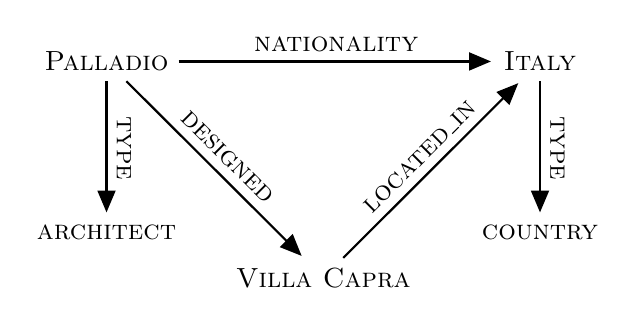
\begin{tikzpicture}[
    ->,
    shorten >=1pt,
    auto,
    node distance=3cm,
    thick,
    main node/.style={draw=none,fill=none}
    ]

    \node[main node] (1) {\entity{Palladio}};
    \node[main node] (2) [right=4cm of 1] {\entity{Italy}};
    \node[main node] (3) [below=1.7cm of 1] {\entity{architect}};
    \node[main node] (4) [below=1.7cm of 2] {\entity{country}};
    \node[main node] (5) [below right=.1cm and .5cm of 3] {\entity{Villa Capra}};

    \path[]
      (1) edge node [sloped, anchor=center, above] {\formalpredicate{nationality}} (2)
      (1) edge node [sloped, anchor=center, above] {\formalpredicate{type}} (3)
      (1) edge node [sloped, anchor=center, above] {\formalpredicate{designed}} (5)
      (2) edge node [sloped, anchor=center, above] {\formalpredicate{type}} (4)
      (5) edge node [sloped, anchor=center, above] {\formalpredicate{located\_in}} (2);
  \end{tikzpicture}
  }
  \textbf{Features between \entity{Palladio} and \entity{Italy}}:\\
  \textless\formalpredicate{nationality}\textgreater\\
  \textless\formalpredicate{designed}$\rightarrow$\formalpredicate{located\_in}\textgreater

  \textbf{Features for \entity{Palladio}}:\\
  \textless\formalpredicate{nationality}\textgreater\\
  \textless\formalpredicate{nationality}\textgreater:\entity{Italy}\\
  \textless\formalpredicate{type}\textgreater:\entity{Architect}\\
  \textless\formalpredicate{designed}$\rightarrow$\formalpredicate{located\_in}\textgreater \\
  \textless\formalpredicate{designed}$\rightarrow$\formalpredicate{located\_in}\textgreater:\entity{Italy}

  \caption{A subset of the Freebase graph, and some example extracted
  features.  The actual Freebase relations and entity identifiers used
  are modified here to aid readability.}
  \label{fig:sfe}
\end{figure}

Subgraph feature extraction (SFE) is a technique introduced by Gardner
and Mitchell~\shortcite{gardner-2015-sfe} for generating feature
matrices over node pairs in a graph with labeled edges.  Given a pair
of nodes in a graph, SFE performs a search to characterize and extract
features from a subgraph around those two nodes.  Example features
include the set of edge sequences that connect the two nodes.
\figref{sfe} shows an example subgraph for the pair \entity{Andrea
Pallado} and \entity{Italy}, and features that would be extracted for
that entity pair.  Gardner and Mitchell used these features to perform
link prediction in the graph, using characteristics of the subgraph
around two nodes to determine if an edge of a particular type should
exist between those nodes.\footnote{When the graph corresponds to a
knowledge base like Freebase, this task is also known as knowledge
base completion.}

We differ from the work done by Gardner and Mitchell in two ways.
First, we apply these features to models of natural language, instead
of to the link prediction task.  Second, Gardner and Mitchell only
considered generating feature matrices over node \emph{pairs} in a
graph, with which one can model binary relations.  The natural
language queries we wish to answer also involve unary predicates.  We
thus extend SFE to also generate feature matrices over \emph{nodes} in
a graph, a straightforward extension that is described in
\secref{method}.

\section{Method}
\label{sec:method}

This section presents our approach to open vocabulary semantic
parsing. Our approach follows the same structure as described in
Section \ref{sec:jayant-semparse}: we generate a surface logical form
from a query, then evaluate it against a probabilistic database with
learned predicate instance probabilities. Section \ref{sec:better-lfs}
describes our logical form generation, which improves the analyses of
noun-mediated relations relative to prior work. Sections
\ref{sec:formal-and-distributional} and \ref{sec:feature-generation}
describe our predicate models and the corresponding feature generation
process. Finally, Section \ref{sec:better-candidates} describes an
improvement on candidate entity generation for question answering.

\subsection{Logical form generation}
\label{sec:better-lfs}

As done by Krishnamurthy and
Mitchell~\shortcite{krishnamurthy-2015-semparse-open-vocabulary}, we
generate logical forms from natural language statements by computing a
syntactic CCG parse, then applying a collection of rules to produce
logical forms. However, their logical form analyses do not model
noun-mediated relations well. For example, given the phrase ``Italian
architect Andrea Palladio,'' their system's logical form would include
the relation $\lexicalpredicate{N/N}(\entity{Italy}, \entity{Andrea
Palladio})$. Here, the \lexicalpredicate{N/N} predicate represents a
generic noun modifier relation; however, this relation is too vague
for the predicate model to accurately learn its denotation. A similar
problem occurs with prepositions and possessives, e.g., it is
similarly hard to learn the denotation of the predicate
\lexicalpredicate{of}.

Our system improves the analysis of noun-mediated relations by simply
including the noun in the predicate name. In the architect example
above, our system produces the relation
\lexicalpredicate{architect\_N/N}. It does this by
concatenating all intervening noun modifiers between two entity
mentions and including them in the predicate name; for example,
``Illinois attorney general Lisa Madigan'' produces the predicate
\lexicalpredicate{attorney\_general\_N/N}).\footnote{While it would be
preferable to use actual dependency relations to determine which words
to add to the predicate, this is not possible because our parser
produces flat analyses of noun phrases where all noun modifiers depend
directly on the head of the noun phrase.} We similarly improve the
analyses of prepositions and possessives to include the head noun. For
example, ``Barack Obama, president of the U.S.'' produces the
predicate instance $\lexicalpredicate{president\_of}(\entity{Barack
  Obama}, \entity{U.S.})$, and ``Rome, Italy's capital'' produces the
predicate \lexicalpredicate{'s\_capital}. This process generates more
specific predicates that we empirically found were easier for the
predicate models to learn.


% While we largely follow the semantic parsing framework introduced by K\&M, we
% made one important change in how logical forms are generated.  For the running
% example we have been using this paper, ``Italian architect Andrea Palladio'',
% the relation predicate produced by K\&M's system is
% $\lexicalpredicate{N/N}(\entity{Italy}, \entity{Andrea Palladio})$.
% \lexicalpredicate{N/N}
% does correctly capture the fact that \entity{Italy} is used syntactically as a
% noun modifier of \entity{Andrea Palladio}, but it leaves out the additional
% information contained in the syntax that ``architect'' was mediating that
% noun-noun dependency.  This means that ``U.S. president Barack Obama'' and
% ``Italian architect Andrea Palladio'' are both modeled using the same relation
% predicate, which leads to a very generic and largely useless model for the
% predicate \lexicalpredicate{N/N}.  By splitting \lexicalpredicate{N/N} into separate
% predicates (\lexicalpredicate{architect\_N/N} and \lexicalpredicate{president\_N/N}), we give
% the model the opportunity to learn more fine-grained relation semantics, and we
% allow our feature selection pipeline to find much more useful features for
% relation predicates.  While it would be ideal to use actual dependency
% relations to determine which words to add to the predicate in complex noun
% phrases, most current parsers treat these kinds of noun phrases as flat, with
% all noun modifiers depending directly on the head of the noun phrase.  We
% approximate this ideal by simply taking all words in between the two entities
% in a noun phrase as the predicate (e.g., ``Illinois attorney general Lisa
% Madigan'' would produce the predicate \lexicalpredicate{attorney\_general\_N/N}).

% A similar issue arises with prepositions and possessives.  For a phrase such as
% ``Barack Obama, president of the U.S.'', K\&M's system would produce the
% following relation predicate: $\lexicalpredicate{of}(\entity{Barack Obama},
% \entity{U.S.})$.  Because this same predicate (\lexicalpredicate{of}) is used for all
% instances of this preposition, the predicate is forced to model too much and
% becomes overly generic.  When there is a common noun mediating a prepositional
% dependency between two entities, as in the phrase above, we add that noun to
% the predicate, giving the instance $\lexicalpredicate{president\_of}(\entity{Barack
% Obama}, \entity{U.S.})$.  We do the same for possessives in phrases such as
% ``Rome, Italy's capital'', producing the predicate \lexicalpredicate{'s\_capital}.

\subsection{Predicate models}
\label{sec:formal-and-distributional}

The key question in the semantic parsing framework we are using is how
to define the predicate models that underlie the probabilistic
database described in \secref{jayant-semparse}.  This is where
previous work used purely distributional models, and where we wish to
include structured information from a knowledge base to improve the
semantics of these predicate models.

We inject information from a knowledge base into our predicate models
by augmenting the learned embeddings with features. In our models, the
truth probability of a category instance $c(e)$ or relation instance
$r(e_1, e_2)$ is given by:

\begin{align*}
  P(c(e)) &= \sigma ( \theta_c^T \phi_e + \omega_c^T \psi_c(e)) \\
  P(r(e_1, e_2)) &= \sigma ( \theta_r^T \phi_{(e_1, e_2)} + \omega_r^T \psi_r(e_1, e_2) )
\end{align*}

In the above equation, the $\theta$ and $\phi$ terms are learned
predicate and entity embeddings, as described in Section
\ref{sec:jayant-semparse}. The second term in the sum represents our
new features and their learned weights. $\psi_c(e)$ and $\psi_r(e_1,
e_2)$ are SFE feature vectors for each entity and entity pair; a
different set of features is chosen for each predicate $c$ and $r$ in
order to maximize their usefulness. The terms $\omega_c$ and
$\omega_r$ represent learned weights for these features.

Each SFE feature can be viewed as either a Freebase query or a horn
clause implication rule using the Freebase schema. In both cases, the
feature defines a set of entities (or entity pairs), and the
associated feature weight measures the likelihood that an entity in
this set is also in the denotation of the surface predicate. Our
models include \emph{many} such features for each surface predicate,
effectively mapping each surface predicate onto a \emph{weighted
  combination of Freebase queries}. This approach is fundamentally
different from typical semantic parsers that map language to a single
Freebase query.

In our model, there are now three sets of parameters to be learned:
(1) $\theta$, low-dimensional distributional vectors trained for each
predicate; (2) $\phi$, low-dimensional distributional vectors trained
for each entity and entity pair; and (3) $\omega$, weights associated
with the selected formal SFE features for each predicate.  All of
these parameters are optimized jointly, using the semantic parsing
framework described in \secref{jayant-semparse}.

\subsection{Generating predicate features}
\label{sec:feature-generation}

The feature vectors $\psi_c(e)$ and $\psi_r(e_1, e_2)$ are constructed
using a two-stage process. First, we generate a predicate-independent
feature vector $\psi(e)$ for each entity $e$ and $\psi(e_1, e_2)$ for
each entity pair $(e_1, e_2)$ using SFE. This step generates very
high-dimensional feature vectors, where most of the
features are not relevant for any given predicate. Next, we perform
per-predicate feature selection to identify a subset of these features
that are relevant for each category and relation predicate.

The predicate-independent feature extraction stage computes the
following feature vectors. For entity pairs, the vector $\psi(e_1,
e_2)$ is a sparse binary vector containing indicator features for all
edge sequences that connect nodes $e_1$ and $e_2$ in the Freebase
graph, up to length 4.  For an entity $e$, the vector $\psi(e)$
contains two kinds of indicator features: (1) all edge sequences up to
length two that begin at $e$, and (2) the same sequences paired with
the entity at their endpoint. Features of type (1) capture the kinds
of relations that an entity participates in, e.g., designing
architectural structures, while features of type (2) capture relations
to other particular entities. This second kind of feature is most
helpful when the endpoint entity is a type, such as
\entity{architect}, although there are some other valuable features of
this kind. \figref{sfe} shows some example entity and entity pair
features extracted from a subset of the Freebase graph.

The feature selection step uses pointwise mutual information (PMI) to
reduce the number of features considered by the model for each
predicate. The feature vectors generated above have tens of millions
of dimensions, but, for any given surface predicate, only a handful of
these dimensions represent relevant Freebase queries. We select
features by first summing the entity and entity pair feature vectors
seen with each predicate in the training data. For example, the phrase
``Italian architect Andrea Palladio'' is considered a positive
training example for the instantiated predicates
$\formalpredicate{architect}(\entity{Andrea Palladio})$ and
$\formalpredicate{architect\_N/N}(\entity{Italy}, \entity{Andrea
Palladio})$. We then add the feature vectors for \entity{Andrea
Palladio} and (\entity{Italy}, \entity{Andrea Palladio}) to the
feature counts for the predicates \formalpredicate{architect} and
\formalpredicate{architect\_N/N}, respectively. This gives a set of
counts \formalpredicate{count}($\pi$), \formalpredicate{count}($f$),
and \formalpredicate{count}($\pi\land f$), for each predicate $\pi$
and feature $f$.  The features are then ranked by PMI for each feature
by computing $\frac{\formalpredicate{count}(\pi\land
f)}{\formalpredicate{count}(\pi)\formalpredicate{count}(f)}$.  After
removing features with counts below a threshold, we pick the $k=100$
features with the highest PMI values for each predicate to use in our
model.

\subsection{Candidate entity generation}
\label{sec:better-candidates}

A key benefit of our predicate models is that they are able to assign
scores to entity pairs that were never seen in the training data. The
purely distributional model of Krishnamurthy and Mitchell has no basis
for assigning these scores and therefore assumes $P(r(e_1,e_2)) = 0$
for unseen entity pairs $(e_1,e_2)$. This assumption limits the recall
of their system when it is applied to question answering, as these
entity pairs will not have been observed for many correct, but rare
entity answers. In contrast, our predicate models can score any entity
pair: the distributional component of an unseen pair will be zero, but
the SFE component is always applicable. This benefit allows our model
to considerably improve question answering performance on rare
entities.

However, this benefit has an associated drawback: given a logical form
query, it is computationally and statistically undesirable to consider
\emph{all} Freebase entities as answers. Scoring millions of entities
is slow, and furthermore makes it more difficult to identify correct
answers (as their relative frequency in the candidate set decreases).
Therefore, when answering a query, we compute a set of candidate
entities and only score these candidates. Our candidate set consists
of all entities seen with the query entities in the training set as
well as all entities directly connected to the query entities in
Freebase, or connected by a mediator node.\footnote{Mediators in
Freebase are used to capture relations with more than two arguments,
such as employment tenure, which has an employer, and employee, a
start date, and an end date.}

Unfortunately, for some entities, such as the United States, the set
of connected entities can be intractably large; we therefore limit
this expansion to only those entities with fewer than 100 directly
connected entities.  Our motivation for this is that this candidate
entity generation is most useful for rarely seen entities, for which
we have few or no related entities seen during training.  These
entities also tend to have relatively few connected entities in
Freebase.

\section{Evaluation}
\label{sec:evaluation}

We evaluate our open-vocabulary semantic parser on a fill-in-the-blank
natural language query task.  Each test example is a natural language
phrase containing at least two Freebase entities, one of which is held
out.  The system must propose a ranked list of Freebase entities to
fill in the blank left by the held out entity, and the predicted
entities are then judged manually for correctness.  We compare our
proposed models, which combine distributional and formal elements,
with a purely distributional baseline from prior work.  All of the
data and code used in these experiments is available at [url withheld
for review].

\subsection{Data}

We use the dataset introduced by Krishnamurthy and
Mitchell~\shortcite{krishnamurthy-2015-semparse-open-vocabulary},
which consists of the ClueWeb09 web
corpus\footnote{http://www.lemuproject.org/clueweb09.php} along with
Google's FACC entity linking of that corpus to
Freebase~\cite{gabrilovich-2013-clueweb-entity-linking}.  For training
data, 3 million webpages from this corpus were processed with a CCG
parser to produce logical forms~\cite{krishnamurthy-2014-joint-ccg}.
This produced 2.1m predicate instances involving 142k entity pairs and
184k entities.  After removing infrequently-seen predicates (seen
fewer than 6 times), there were 25k categories and 4.2k
relations.\footnote{The differences in numbers reported here versus
those reported by Krishnamurthy and
Mitchell~\shortcite{krishnamurthy-2015-semparse-open-vocabulary} are
due to our improved logical form generation, discussed in
\secref{better-lfs}.}

We also used the test set created by Krishnamurthy and Mitchell, which
contains 220 queries generated in the same fashion as the training
data from a separate section of ClueWeb.  However, as they did not
release a development set with their data, we used this set as a
development set.  For a final evaluation, we generated another,
similar test set from a different held out section of ClueWeb, in the
same fashion as done by Krishnamurthy and Mitchell.  This final test
set contains 307 queries.  We report results on both of these sets
below.

\subsection{Models}

We compare three models in our experiments: (1) a distributional model
(the prior work of Krishnamurthy and
Mitchell~\shortcite{krishnamurthy-2015-semparse-open-vocabulary}); (2)
a formal model (new to this work), where the distributional parameters
$\theta$ and $\phi$ in \secref{formal-and-distributional} are fixed at
zero; and (3) the combined model described in
\secref{formal-and-distributional} (also new to this work).  Except
where noted, all experiments use our modified logical forms
(\secref{better-lfs}) and our entity proposal mechanism
(\secref{better-candidates}).

\subsection{Methodology}

Given a fill-in-the-blank query such as ``Italian architect
\blank{}'', each system produces a ranked list of 100 candidate
entities.  To compare the output of the systems, we follow a pooled
evaluation protocol commonly used in relation extraction and
information
retrieval~\cite{west-2014-kbc-via-qa,riedel-2013-mf-universal-schema}.
We take the top 30 predictions from each system and manually annotate
whether they are correct, and use those annotations to compute the
average precision (AP) and reciprocal rank (RR) of each system on the
query.  Average precision is defined as $\frac{1}{m}\sum^m_{k=1}
\mathrm{Prec}(k) \times \mathrm{Correct}(k)$, where $\mathrm{Prec}(k)$
is the precision at rank $k$, $\mathrm{Correct}(k)$ is an indicator
function for whether the $k$th answer is correct, and $m$ is number of
returned answers (up to 100 in this evaluation).  AP is equivalent to
calculating the area under a precision-recall curve.  Reciprocal rank
is computed by first finding the rank $r$ of the first correct
prediction made by a system.  Reciprocal rank is then $\frac{1}{r}$,
ranging from 1 (if the first prediction is correct) to 0 (if there is
no correct answer returned).  In the tables below we report
\emph{mean} average precision (MAP) and \emph{mean} reciprocal rank
(MRR), averaged over all of the queries in the test set.  We also
report a weighted version of MAP, where the AP of each query is scaled
by the number of annotated correct answers to the query (shown as
W-MAP in the tables for space considerations).

\subsection{Results}

\begin{table}
  \centering
  {\small
    \begin{tabular}{lcc}
      \toprule
      Method & K\&M's LFs & Our LFs \\
      \midrule
      Distributional model & .269 & \textbf{.284} \\
      \midrule
      Formal model & .231 & \textbf{.276} \\
      \midrule
      Combined model & .313 & \textbf{.335} \\
      \bottomrule
    \end{tabular}
  }
  \caption{Comparison of models using logical forms from prior work
  versus those introduced in this paper.  The metric shown is mean
  average precision on the dev set.  With our logical forms,
  performance of all models improves, quite substantially in the case
  of the formal model.}
  \label{tab:better-lfs}
\end{table}

We first show the effect of using the new logical forms introduced in
\secref{better-lfs}.  As can be seen in \tabref{better-lfs}, with
improved logical forms, all models are better able to capture the
semantics of language.  This improvement is more pronounced in the
formal models, which have more capacity to get specific features from
Freebase with the new logical forms.  As our logical forms are able to
give all models better performance, the remaining experiments we
present all use these logical forms.

\begin{table}
  \centering
  {\small
    \begin{tabular}{lccc}
      \toprule
      Method & MAP & W-MAP & MRR \\
      \midrule
      Distributional model & .163 & .163 & .288 \\
      \midrule
      With freebase entities & .\textbf{229} & \textbf{.275} & \textbf{.312} \\
      \midrule
      \midrule
      Relative improvement & 40\% & 69\% & 8\% \\
      \bottomrule
    \end{tabular}
  }
  \caption{Allowing Krishnamurthy and Mitchell's model to propose
  candidate entities from Freebase improves mean average precision
  substantially, by allowing the model to have higher recall.}
  \label{tab:better-candidates}
\end{table}

We next show the improvement gained by using the simple candidate
entity generation outlined in \secref{better-candidates}.  By simply
appending the list of connected entities in Freebase to the end of the
rankings returned by the distributional model, MAP improves by 40\%
(see \tabref{better-candidates}).  The connectedness of an entity pair
in Freebase is very informative, especially for rare entities that are
not seen together during training.

\begin{table}
  \centering
  {\small
    \begin{tabular}{lccc}
      \toprule
      Method & MAP & W-MAP & MRR \\
      \midrule
      Prior work (distributional) & .284 & .371 & .379 \\
      \midrule
      Our formal model & .276 & .469 & .334 \\
      \midrule
      Our combined model & \textbf{.335} & \textbf{.477} & \textbf{.429} \\
      \midrule
      \midrule
      Relative improvement & 18\% & 29\% & 13\% \\
      \bottomrule
    \end{tabular}
  }
  \caption{Results on the development set for our fill-in-the-blank task.  The
  combined model significantly improves MAP over prior work.}
  \label{tab:dev-results}
\end{table}

\tabref{dev-results} shows a comparison between the semantic parsing
models we have discussed on the development set.  As can be seen, the
combined model significantly improves performance over prior work,
giving a relative gain in weighted MAP of 29\%.

\begin{table}
  \centering
  {\small
    \begin{tabular}{lccc}
      \toprule
      Method & MAP & W-MAP & MRR \\
      \midrule
      Prior work (distributional) & .229 & .275 & .312 \\
      \midrule
      Our formal model & .355 & .495 & .419 \\
      \midrule
      Our combined model & \textbf{.370} & \textbf{.513} & \textbf{.469} \\
      \midrule
      \midrule
      Relative improvement & 62\% & 87\% & 50\% \\
      \bottomrule
    \end{tabular}
  }
  \caption{Results on the final test set for our fill-in-the-blank
  task.  The combined model improves over prior work by 50--87\% on
  our metrics.  Note that these improvements over the baseline are
  \emph{after} the baseline has been improved by the methods developed
  in this paper, shown in \tabref{better-lfs} and
  \tabref{better-candidates}.  The cumulative effect of the methods
  presented in this work is an improvement of over 120\% in MAP.}
  \label{tab:final-results}
\end{table}

\tabref{final-results} shows that these improvements are consistent on
the final test set, as well.  The performance improvement seen by the
combined model is actually larger on this set, with gains on our
metrics ranging from 50\% to 87\%.

On both of these datasets, the difference in MAP between the combined
model and the distributional model is statistically significant (by a
paired permutation test, $p < 0.05$).  The differences between the
combined model and the formal model, and between the formal model and
the distributional model, are not statistically significant, as each
method has certain kinds of queries that it performs well on.  Only
the combined model is able to consistently outperform the
distributional model on all kinds of queries.

\subsection{Discussion}

Our model tends to outperform the distributional model on queries
containing predicates with exact or partial correlates in
Freebase. For example, our model obtains nearly perfect average
precision on the queries ``French newspaper \blank{}'' and ``Israeli
prime minister \blank{},'' both of which can be exactly expressed in
Freebase.  The top features for \lexicalpredicate{newspaper}($x$) all
indicate that $x$ has type \formalpredicate{newspaper} in Freebase,
and the top features for \lexicalpredicate{newspaper\_N/N}($x$, $y$)
indicate that $y$ is a newspaper, and that $x$ is either the
circulation area of $y$ or the language of $y$.

The model also performs well on queries with partial Freebase
correlates, such as ``Microsoft head honcho \blank{}'', ``The United
States, \blank{}'s closest ally'', and ``Patriots linebacker
\blank{},'' although with somewhat lower average precision. The high
weight features in these cases tend to provide useful hints, even
though there is no direct correlate; for example, the model learns
that ``honchos'' are people, and that they tend to be CEOs and film
producers.

There are also some areas where our model can be improved. First, in
some cases, the edge sequence features used by the model are not
expressive enough to identify the correct relation in Freebase. An
example of this problem is the ``linebacker'' example above, where the
features for \lexicalpredicate{linebacker\_N/N} can capture which athletes
play for which teams, but not the \emph{positions} of those
athletes. Second, our model can underperform on predicates with no
close mapping to Freebase. An example where this problem occurs is the
query ``\blank{} is a NASA mission.'' Third, there remains room to
further improve the logical forms produced by the semantic parser,
specifically for multi-word expressions. One problem occurs with
multi-word noun modifiers, e.g., ``Vice president Al Gore'' is mapped
to $\lexicalpredicate{vice}(\entity{Al Gore}) \land
\lexicalpredicate{president}(\entity{Al Gore})$. Another problem is that
there is no backoff with multi-word relations. For example, the
predicate \lexicalpredicate{head\_honcho\_N/N} was never seen in the training
data, so it is replaced with \lexicalpredicate{unknown}; however, it would be
better to replace it with \lexicalpredicate{honcho\_N/N}, which \emph{was}
seen in the training data. Finally, although using connected entities
in Freebase as additional candidates during inference is helpful, it
often over- or under-generates candidates. A more tailored, per-query
search process could improve performance.

\section{Related work}

In addition to the work described in \secref{background}, there are
three broad classes of work that are related to what we have presented
in this paper.

The first line of research that our work is related to is knowledge
base completion.  In addition to SFE~\cite{gardner-2015-sfe}, our work
draws inspiration from work on embedding the entities and relations in
a knowledge base~\cite{riedel-2013-mf-universal-schema,%
nickel-2011-rescal,bordes-2013-transe,nickel-2014-are,%
toutanova-2015-joint-text-kb-embedding}, as well as work on
graph-based methods for reasoning with knowledge
bases~\cite{lao-2010-original-pra,gardner-2014-vector-space-pra,%
neelakantan-2015-rnn-kbc}.

Second, our work is conceptually related to many methods that aim to
learn word embeddings that are informed by some kind of external
knowledge~\cite{faruqui-2015-retrofitting-word-vectors,%
rocktaschel-2015-logical-embeddings,schwartz-2016-symmetric-patterns-w2v,%
yu-2014-w2v-with-semantic-knowledge}.  A key difference between these
approaches and ours is that they use the structured information only
to modify distributional representations, while we include the
structured information directly in our models, training feature
weights jointly with distributional representations.

Lastly, there is an extensive literature on building semantic parsers
to answer questions against a structured knowledge
base~\cite{zettlemoyer-2005-ccg,berant-2013-semantic-parsing-qa,%
kwiatkowski-2013-ontology-matching,krishnamurthy-2012-semantic-parsing,%
li-2015-semantic-parsing-scfg}.  The vast majority of this work is
focused on matching natural language text to statements in a specific
schema, with no hope of assigning meaning to language that falls
outside of that schema.  Only very recently has there been work
attempting to learn broad coverage meaning representations in semantic
parsers.  In addition to the work by Krishnamurthy and Mitchell
discussed in \secref{background}, and work by Lewis and
Steedman~\shortcite{lewis-2013-combined-distributional-and-logical-semantics}
which Krishnamurthy and Mitchell extended, Choi et
al.~\shortcite{choi-2015-semantic-parsing-partial-ontologies},
extended a traditional semantic parser with the notion of ``open''
predicates not contained in the Freebase ontology.  A key difference
between their work and ours is that, while their system might learn
that ``front-runner'' should be modeled as an open predicate that has
no representation in Freebase, they have no method to assign any
further meaning to that predicate, whereas our models learn both
distributional and formal information about the meaning of
``front-runner''.

\section{Conclusion}
\label{sec:conclusion}

This paper considers the problem of assigning meaning to predicates
(both categories and relations) in natural language using both
distributional information and information from a formal knowledge
base. Our model represents words as a weighted combination of
knowledge base queries plus a distributional component. Both of these
components are jointly trained to correctly predict entity answers to
fill-in-the-blank natural language queries. This combined model
achieved relative gains of over 50\% in mean average precision and
mean reciprocal rank versus a purely distributional approach.  We also
introduced a better mapping from surface text to logical forms, and a
simple method for using Freebase to find candidate entities during
inference.  Taken together, the methods introduced in this paper
improved mean average precision on our task from .163 to .370, a 127\%
relative improvement over prior work.

A consequence of this work is that it suggests a new direction for
semantic parsing research. Existing semantic parsers map language to a
single knowledge base query, an approach that successfully leverages a
knowledge base's predicate instances, but is fundamentally limited by
its schema. In contrast, our approach maps language to a
\emph{weighted combination of queries} plus a distributional
component; this approach is capable of representing a much broader
class of concepts while still using the knowledge base when it is
helpful. Furthermore, it is capable of using the knowledge base even
when the meaning of the language cannot be exactly represented by a
knowledge base predicate, which is a common occurrence. We believe
that this kind of approach could significantly expand the
applicability of semantic parsing techniques to more complex domains
where the assumptions of traditional techniques are too limiting.

%\section*{Acknowledgments}

\bibliography{bib}
\bibliographystyle{acl2016}

\end{document}
